\documentclass[12pt]{article}
\usepackage[utf8]{inputenc}

\title{Specyfikacja implementacyjna}
\author{Patryk Zaniewski}
\date{11.11.2018}

\usepackage{natbib}
\usepackage{graphicx}
\usepackage{polski}
\usepackage{indentfirst}
\usepackage{geometry}

\begin{document}

\maketitle

\tableofcontents
\newpage

\section{Wstęp}
Problemem poruszanym przez program jest rynek wymian walut. Pięciu spekulantów potrzebuje programu, który w prosty sposób pomoże im osiągnąć jak największy zysk. Oczekują oni, że dostarczony im program będzie realizował dwie funkcje. Pierwszą z nich jest wyznaczanie ścieżki wymiany walut. Dodatkowo, taka ścieżka musi być jak najbardziej dochodowa dla użytkownika. Drugą z funkcji jest możliwość wyznaczenia dowolnego arbitrażu walutowego na podstawie ilości pieniędzy przez niego posiadanych.

\section{Wykorzystane technologie oraz środowisko programistyczne i sprzętowe}
Do napisania programu zostanie wykorzystany język Java w wersji 11. Projekt będzie realizowany w środowisku programistycznym Intellij Idea 2018 firmy JetBrains. Program będzie pisany oraz testowany na dwóch komputerach o następujących parametrach.

\begin{itemize}
\item  Intel Core i7 2600K 4.1GHz, 8GB DDR3 1600MHz, ASRock Z77 Extreme4, Windows 7 Ultimate,
\item  Intel Core i5 2.6 GHz, 8GB DDR3 1600MHz, MacOS Mojave.
\end{itemize}

\section{Opis wykorzystanych algorytmów}
Program poza standardowymi algorytmami wczytywania, walidacji oraz wypisywania danych będzie zawierał szereg innych algorytmów. Odpowiedzialne one będą za właściwe przekazywanie kursów walut do struktury grafu, wyszukiwanie najkorzystniejszej ścieżki wymiany waluty wejściowej na wyjściową oraz za wyszukiwanie arbitrażu walutowego.
\newline\newline
Algorytm przekazywania i umieszczania danych w strukturze będzie opierał się na liście list, a co za tym idzie, na grafie. Każda z walut będzie posiadała własną listę sąsiadów z której będzie można odczytać do jakiej innej waluty wyjściowej możemy przewalutować aktualną walutę. Dodatkowo, graf będzie zawierał informacje o kursach między walutami oraz o opłatach ponoszonych przy wymianie.
\newline\newline
Algorytmem odpowiedzialnym za wyszukiwanie najkorzystniejszej ścieżki wymiany walut będzie algorytm Bellmana-Forda. Jednak dla jego poprawnego działania należy wszystkie koszty przewalutowań przedstawić w postaci: \textbf{1/koszt przewalutowania}. Sprawi to, że algorytm wyznaczy najkrótszą ścieżkę w grafie dla odwróconych liczb (jeśli jest ona możliwa), a co za tym idzie największy mnożnik przewalutowania między walutą wejściową, a wyjściową.
\newline\newline
Algorytmem odpowiedzialnym za wyszukiwanie arbitrażu walutowego również będzie algorytm Bellmana-Forda. Jednak w tym przypadku wyszukiwanie najkrótszych ścieżek nie będzie jego głównym zadaniem. Jego celem będzie zwrócenie ścieżki wymiany w której nastąpił arbitraż.

\section{Diagram klas}
Na poniższym diagramie \emph{Rysunek 1} zostały zobrazowane zależności między klasami w programie. Każda z klas wraz z jej metodami zostanie opisana w kolejnym punkcie.

\begin{figure}[h!]
\centerline{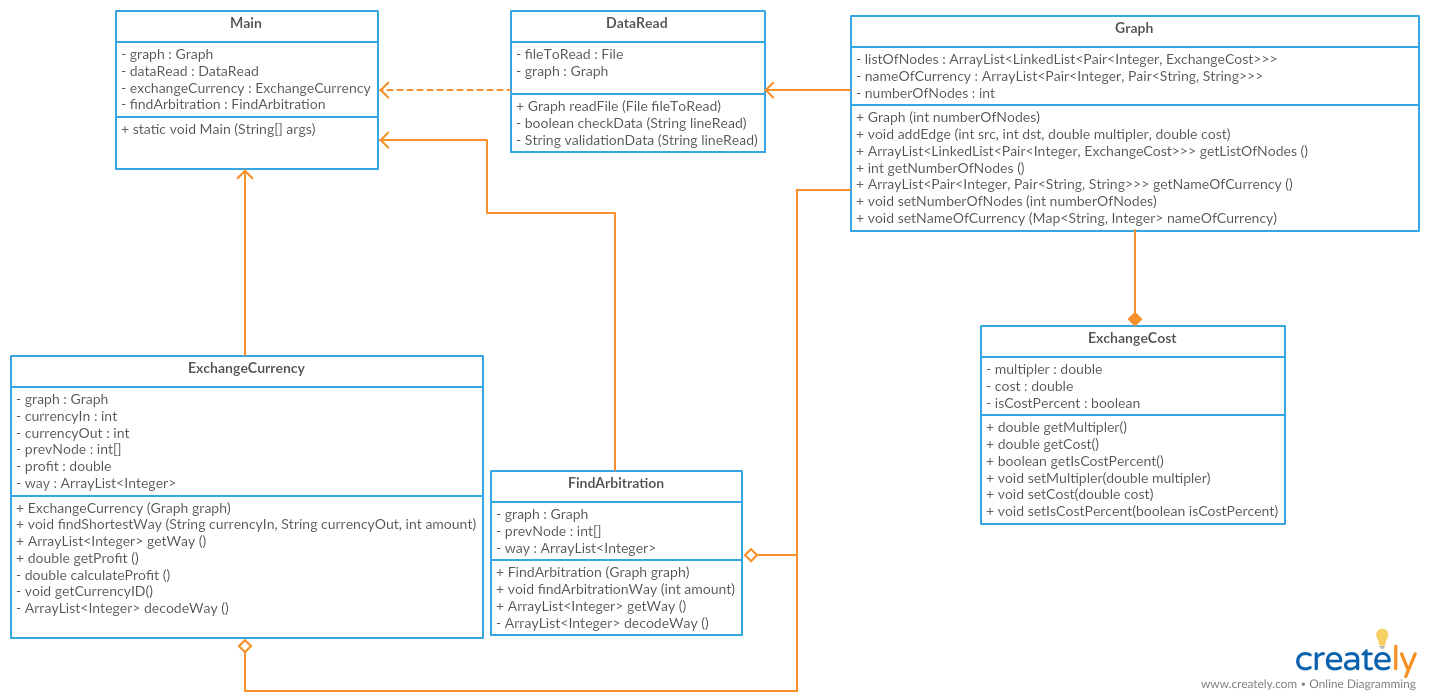
\includegraphics[scale=0.37]{diagram}}
\caption{diagram klas}
\label{fig:diagram}
\end{figure}

\section{Opis klas i metod}
W programie znajduje się 6 klas: Main, DataRead, Graph, ExchangeCost, FindArbitration oraz ExchangeCurrency. Poniżej zostały wymienione oraz opisane wszystkie przewidywane pola i metody. Pominięte zostały metody get() i set() z uwagi na ich oczywiste przeznaczenie.
\begin{enumerate}
\item \textbf{Main} - główna klasa rozpoczynająca program. Będzie odpowiadała za wczytywanie danych oraz za komunikację z użytkownikiem. Klasa będzie zawierać następujące pola:
    \begin{itemize}
        \item \begin{verbatim}private Graph graph\end{verbatim}
        zmienna odpowiedzialna za przechowanie grafu zwróconego przez klasę DataRead po wczytaniu danych,
    \item \begin{verbatim}private DataRead dataRead\end{verbatim}
        zmienna odpowiedzialna za przechowanie obiektu klasy wczytującej dane,
    \item \begin{verbatim}private ExchangeCurrency exchangeCurrency\end{verbatim}
        zmienna odpowiedzialna za przechowywanie obiektu klasy ExchangeCurrency na której wykonywane są operacje wyszukiwania korzystnej ścieżki,
    \item \begin{verbatim}private FindArbitration FindArbitration\end{verbatim}
        zmienna odpowiedzialna za przechowywanie obiektu klasy FindArbitration na której wykonywane są operacje wyszukiwania dowolnego arbitrażu walutowego.
    \end{itemize}
    oraz metody:
    \begin{itemize}
        \item \begin{verbatim}public static void main (String [] args)\end{verbatim}
        główna metoda rozpoczynająca i sterująca działaniem programu.
    \end{itemize}
\item \textbf{DataRead} - klasa odpowiedzialna za wczytywanie danych oraz ich walidację. Klasa będzie zawierać następujące pola:
    \begin{itemize}
        \item \begin{verbatim}private File fileToRead\end{verbatim}
        zmienna odpowiedzialna za przechowywanie pliku z którego następuje wczytywanie danych,
    \item \begin{verbatim}private Graph graph\end{verbatim}
        zmienna odpowiedzialna za przechowywanie danych w postaci obiektu klasy Graph.
    \end{itemize}
    oraz metody:
    \begin{itemize}
        \item \begin{verbatim}public Graph readFile (File fileToRead)\end{verbatim}
        metoda odpowiedzialna za przeprowadzenie procesu wczytywania danych oraz za utworzenie obiektu klasy Graph,
        \item \begin{verbatim}private boolean checkData (String lineRead)\end{verbatim}
        metoda odpowiedzialna za sprawdzenie poprawności wczytywanej linii danych,
        \item \begin{verbatim}private String validationData (String lineRead)\end{verbatim}
        metoda odpowiedzialna za obsługę źle wprowadzonych danych w linii.
    \end{itemize}
\item \textbf{Graph} - klasa odpowiedzialna za właściwe umieszczenie danych oraz za przechowanie ich w postaci grafu. Klasa będzie zawierać następujące pola:
    \begin{itemize}
        \item \begin{verbatim}private ArrayList<LinkedList<Pair<Integer, ExchangeCost>>> listOfNodes\end{verbatim}
        zmienna odpowiedzialna za przechowanie grafu w postaci listy sąsiedztwa każdego wierzchołka,
    \item \begin{verbatim}private Map<Integer, Pair<String, String>> nameOfCurrency\end{verbatim}
        zmienna odpowiedzialna za przechowywanie skrótów oraz pełnych nazw walut. Każda z tych wartości wywoływana jest na podstawie klucza, którym jest ID waluty,
    \item \begin{verbatim}private int numberOfNodes\end{verbatim}
        zmienna odpowiedzialna za przechowywanie informacji o ilości wierzchołków grafu czyli wczytanych walut.
    \end{itemize}
    oraz metody:
    \begin{itemize}
        \item \begin{verbatim}public Graph (int numberOfNodes)\end{verbatim}
        konstuktor, którego zadaniem jest stworzenie listy list w takiej liczbie ile zostało wczytanych walut,
        \item \begin{verbatim}public void addEdge (int src, int dst, double multipler, double cost)\end{verbatim}
        metoda odpowiedzialna za utworzenie połączenia między dwoma wierzchołkami grafu oraz za ustawienie wagi krawędzi między nimi.
    \end{itemize}
\item \textbf{ExchangeCost} - klasa odpowiedzialna za przechowywanie danych dotyczących kursów walut oraz kosztów wymiany. Klasa zawiera następujące pola:
    \begin{itemize}
        \item \begin{verbatim}private double multipler\end{verbatim}
        zmienna odpowiedzialna za przechowanie stosunku wymiany waluty wejściowej do wyjściowej,
    \item \begin{verbatim}private double cost\end{verbatim}
        zmienna odpowiedzialna za przechowywanie kosztu wymiany waluty wejściowej na wyjściową,
    \item \begin{verbatim}private boolean isCostPercent\end{verbatim}
        zmienna odpowiedzialna za przechowywanie informacji czy po wymianie opłata od waluty wyjściowej jest stała czy procentowa.
    \end{itemize}
\item \textbf{FindArbitration} - klasa odpowiedzialna za wyszukiwanie arbitrażu walutowego. Algorytm wyszukiwania zawarty w tej klasie opiera się na algorytmie Bellmana - Forda, co zostało opisane wyżej. Klasa będzie zawierać następujące pola:
    \begin{itemize}
        \item \begin{verbatim}private Graph graph\end{verbatim}
        zmienna odpowiedzialna za przechowanie grafu wewnątrz którego będzie wyszukiwany arbitraż walutowy,
    \item \begin{verbatim}private int[] prevNode\end{verbatim}
        zmienna odpowiedzialna za przechowywanie informacji o poprzedniku danego wierzchołka,
    \item \begin{verbatim}private ArrayList<Integer> way \end{verbatim}
        zmienna odpowiedzialna za przechowywanie ścieżki arbitrażu.
    \end{itemize}
    oraz metody:
    \begin{itemize}
        \item \begin{verbatim}public FindArbitration (Graph graph)\end{verbatim}
        konstruktor, który przekazuje obiekt typu Graph i przypisuje go do zmiennej graph,
         \item \begin{verbatim}public void findArbitrationWay (int amount)\end{verbatim}
        metoda, która na podstawie podanej ilości dowolnej waluty wyszukuje dowolny arbitraż,
         \item \begin{verbatim}private ArrayList<Integer> findArbitrationWay ()\end{verbatim}
        metoda, która zwraca ścieżkę arbitrażu.
        
    \end{itemize}
\item \textbf{ExchangeCurrency} - klasa odpowiedzialna za wyszukiwanie najkorzystniejszej ścieżki wymiany waluty wejściowej na walutę wyjściową. Algorytm wyszukiwania tak jak algorytm wyszukiwania arbitrażu walutowego opiera się na algorytmie Bellmana - Forda, co zostało opisane wyżej. Klasa będzie zawierać następujące pola:
    \begin{itemize}
        \item \begin{verbatim}private Graph graph\end{verbatim}
        zmienna odpowiedzialna za przechowanie grafu wewnątrz którego będzie wyszukiwana najkorzystniejsza ścieżka wymiany waluty,
    \item \begin{verbatim}private int currencyIn\end{verbatim}
        zmienna odpowiedzialna za przechowywanie wierzchołka wejściowego,
    \item \begin{verbatim}private int currencyOut \end{verbatim}
        zmienna odpowiedzialna za przechowywanie wierzchołka wyjściowego,
    \item \begin{verbatim}private int[] prevNode\end{verbatim}
        zmienna odpowiedzialna za przechowywanie  informacji o poprzedniku danego wierzchołka,
    \item \begin{verbatim}private int profit\end{verbatim}
        zmienna odpowiedzialna za przechowywanie wyniku najkorzystniejszej wymiany waluty,
    \item \begin{verbatim}private ArrayList<Integer> way\end{verbatim}
        zmienna odpowiedzialna za przechowywanie ścieżki arbitrażu.
    \end{itemize}
    oraz metody:
    \begin{itemize}
        \item \begin{verbatim}public ExchangeCurrency (Graph graph)\end{verbatim}
        konstruktor, który przekazuje obiekt typu Graph i przypisuje go do zmiennej graph,
         \item \begin{verbatim}public void findShortestWay (String currencyIn, String currencyOut,
         int amount)\end{verbatim}
        metoda, która na podstawie walut wejściowej i wyjściowej oraz ilości waluty wejściowej wyszukuje najkorzystniejszą ścieżkę wymiany,
         \item \begin{verbatim}private double calculateProfit ()\end{verbatim}
        metoda, która wylicza najkorzystniejszy wynik wymiany walut,
        \item \begin{verbatim}private void getCurrencyID ()\end{verbatim}
        metoda, która na podstawie podanych nazwa walut wyszukuje ich ID oraz zapisuje je w zmiennych currencyIn oraz currencyOut,
        \item \begin{verbatim}private ArrayList<Integer> decodeWay ()\end{verbatim}
        metoda, która zapisuje ścieżkę najkorzystniejszej wymiany walut.
        
    \end{itemize}
\end{enumerate}

\section{Spis zaimportowanych pakietów}
W programie zostaną zaimportowane i użyte pakiety wymienione poniżej. 
\begin{enumerate}
    \item java.lang
    \item java.util
    \item java.io
    
\end{enumerate}

\section{Testy jednostkowe}
Testy jednostkowe generowane będą za pomocą narzędzia JUnit za pomocą którego otrzymamy możliwość sprawdzenia poszczególnych metod w klasach. Przykładowe testy oraz spodziewane rezultaty:
\begin{itemize}
    \item Dane w pliku są wprowadzone w niepoprawny sposób - program po wykryciu błędów zaproponuje trzy opcje: pominięcie linii, jej ręczną edycję lub zakończenie działania programu.
    \item Wybrana przez użytkownika waluta wejściowa lub wejściowa nie istnieje - program wypisze błąd.
    \item Brak możliwości wymiany waluty wejściowej na wyjściową - program wypisze komunikat o braku możliwości wyminy.
    \item Użytkownik poda ujemną kwotę pieniędzy - program wypisze komunikat o błędzie
    \item Program dla poprawnych danych oraz poprawnego zapytania zwróci dane dotyczące wymiany. Przykładowy plik z danymi oraz przykładowe zapytanie:
    \begin{scriptsize}{\begin{verbatim}
    # Waluty (id | symbol | pełna nazwa)
    0 PLN zloty
    1 EUR euro
    2 USD dolar amerykański
    # Kursy walut (id | symbol (waluta wejściowa) | symbol (waluta wyjściowa) | kurs | typ opłaty | opłata
    0 PLN EUR 0,2513 PROC 0,1
    1 PLN USD 0.1323 PROC 0
    2 EUR USD 1,1370 STAŁA 0.025
    
    \end{verbatim}}\end{scriptsize}
    W dalszej kolejności program zostanie poproszony o najkorzystniejszą wymianę poprzez wprowadzenie zapytania:
    \begin{scriptsize}{\begin{verbatim}
    PLN 100 USD
     \end{verbatim}}\end{scriptsize}
    Otrzymanym rezultatem końcowym będzie 25.69. Wynik końcowy zostanie zaokrąglony do części setnych.
    \item Program dla poprawnych danych oraz poprawnego zapytania zwróci dane dotyczące arbitrażu. Przykładowy plik z danymi oraz przykładowe zapytanie:
    \begin{scriptsize}{\begin{verbatim}
    # Waluty (id | symbol | pełna nazwa)
    0 PLN zloty
    1 EUR euro
    2 USD dolar amerykański
    # Kursy walut (id | symbol (waluta wejściowa) | symbol (waluta wyjściowa) | kurs | typ opłaty | opłata
    0 PLN EUR 0,2513 PROC 0,1
    1 USD PLN 0.1323 PROC 0
    2 EUR USD 1,1370 STAŁA 0.025
     \end{verbatim}}\end{scriptsize}
    W dalszej kolejności program zostanie poproszony o arbitraż poprzez wprowadzenie zapytania:
    \begin{scriptsize}{\begin{verbatim}
    100
     \end{verbatim}}\end{scriptsize}
     Otrzymanym rezultatem końcowym będzie wypisanie przez program kolejnych walut arbitrażu czyli:  PLN - EUR - USD - PLN.
    
\end{itemize}
\end{document}
